
\chapter{Muminav}

Beispiel Progamm, welches zeigt wie man Muminav einbinden kann.

relevante andere Projekte - hoch spezifizierte Anforderungen

\section{Lizenz}

Vorgabe war, die gesamte Entwicklungsarbeit als Open Source
Projekt durchzuf�hren. Dies schlie�t ein, die
Projektergebnisse unter einer Open Source Lizenz \cite{OpenSourceLicences} zu ver�ffentlichen.\\
Da wir unser Projekt in Zusammenarbeit mit der Mumie-Gruppe
entwickeln, mussten wir uns im Vorfeld mit Ihnen auf eine Open
Source Lizenz verst�ndigen, welche in das Gesamtprojekt
\textsc{Mumie}
integrierbar ist.\\
Die GPL \cite{GPL} (GNU General Public License)



LGPL \cite{LGPL}.

\section{Entwicklungsumgebung}
\subsection{Enwicklungswerkzeuge}
F�r das Projekt wurden eine Reihe von Entwicklungswerkzeugen und
Technologien verwandt, welche f�r Open-Source-Projekte
charakteristisch sind:

\begin{itemize}

\item \textbf{Malinglisten} blah \ldots
\item \textbf{CVS} \cite{CVSRedbook}
\item \textbf{eMail}
\item \textbf{Instant-Messageing}
\item \textbf{Projekt-Homepage}
\item \textbf{Newsgroups}

%\item \textbf{}
\end{itemize}

Ant \cite{Ant2002}, JBuilder \cite{BerliOS}
\subsection{Projekthoster}

\subsection{Problemen und ihre L�sungen}

XML-Parser mitliefern - Gr��e - Entscheidung f�r Java 1.4 und
Mozilla

\section{Verwendete Komponenten und Ressourcen}

\begin{figure}[htbp]
    \centering%
%   \setcapwidth[c]{12cm}%
    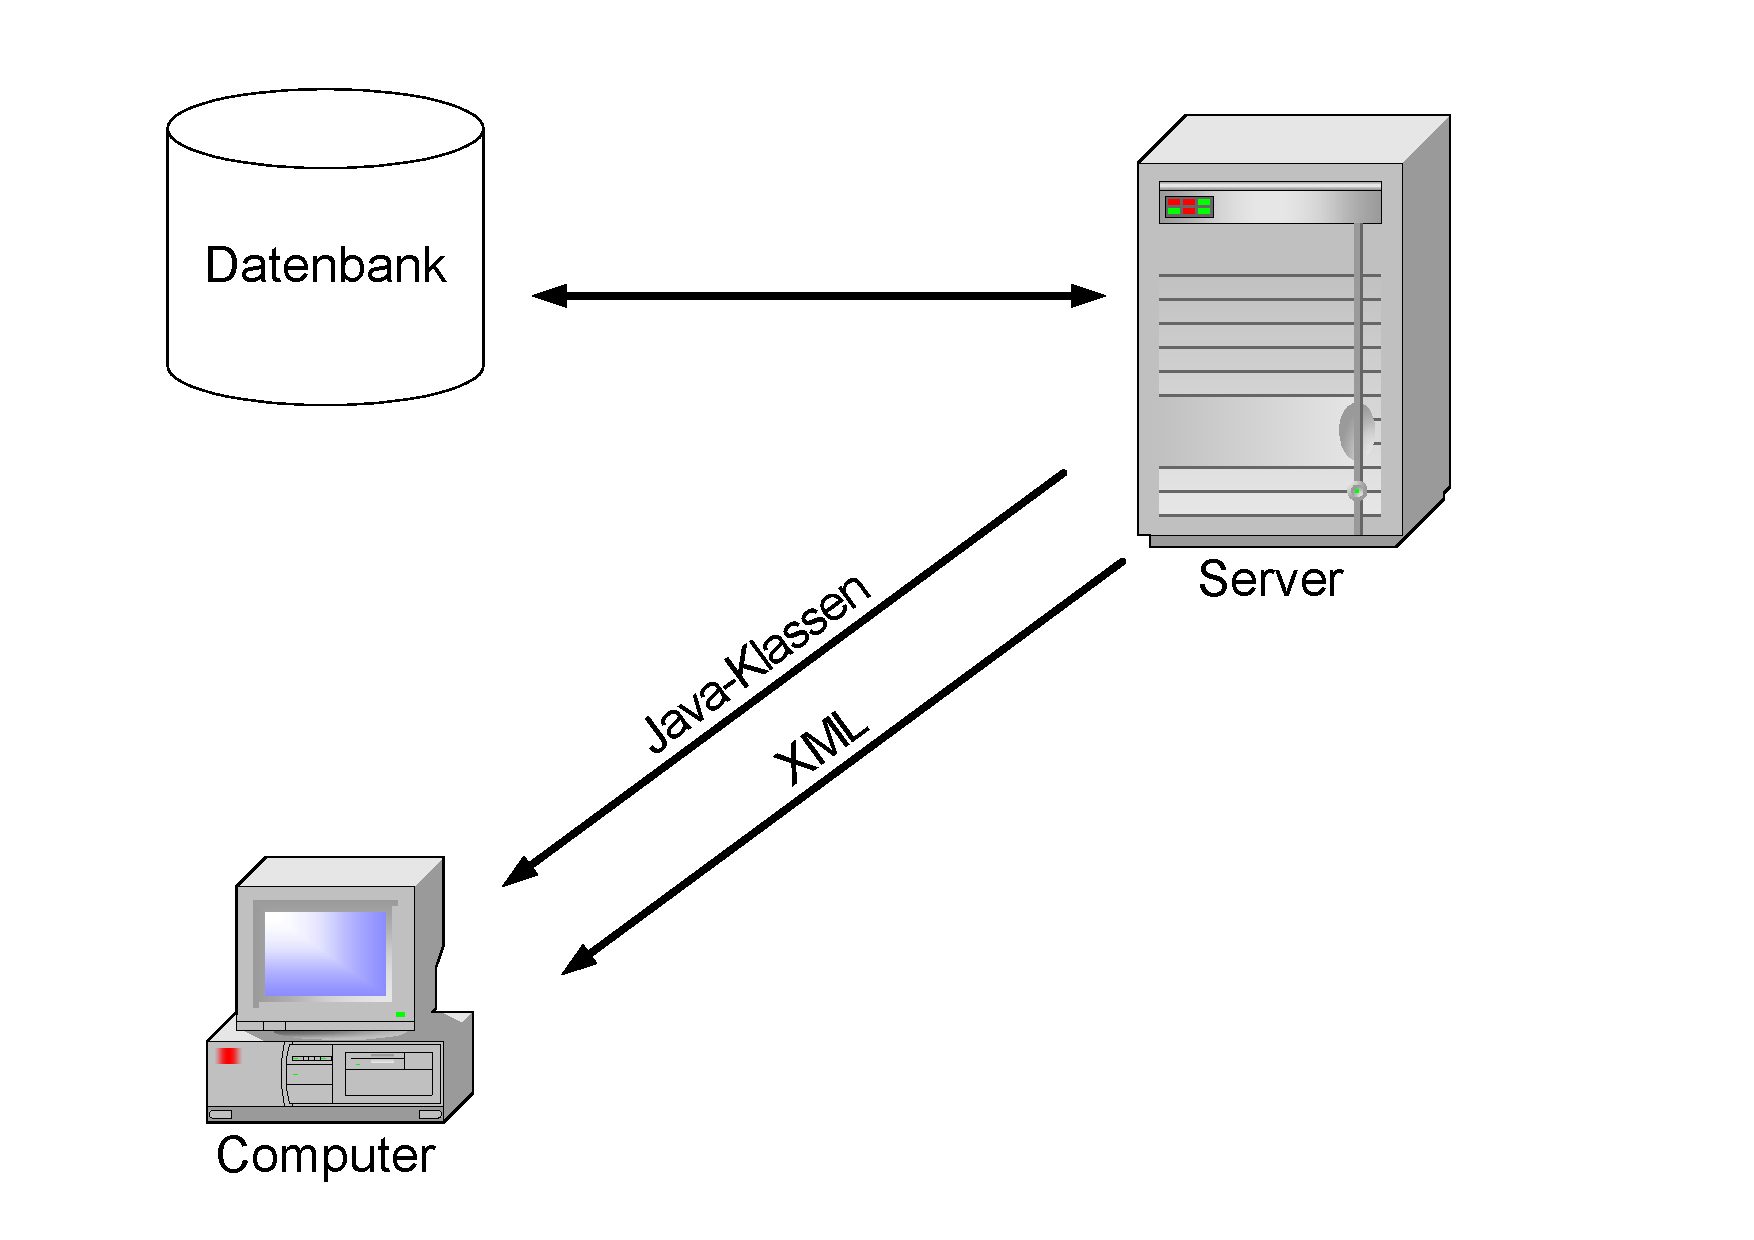
\includegraphics[width=10cm]{figs/kommunikation}
    \captionbelow{Kommunikation: Informationsfluss}
    \label{FIG:kommunikationsfluss}
\end{figure}

\begin{figure}[htbp]
    \centering%
%   \setcapwidth[c]{12cm}%
    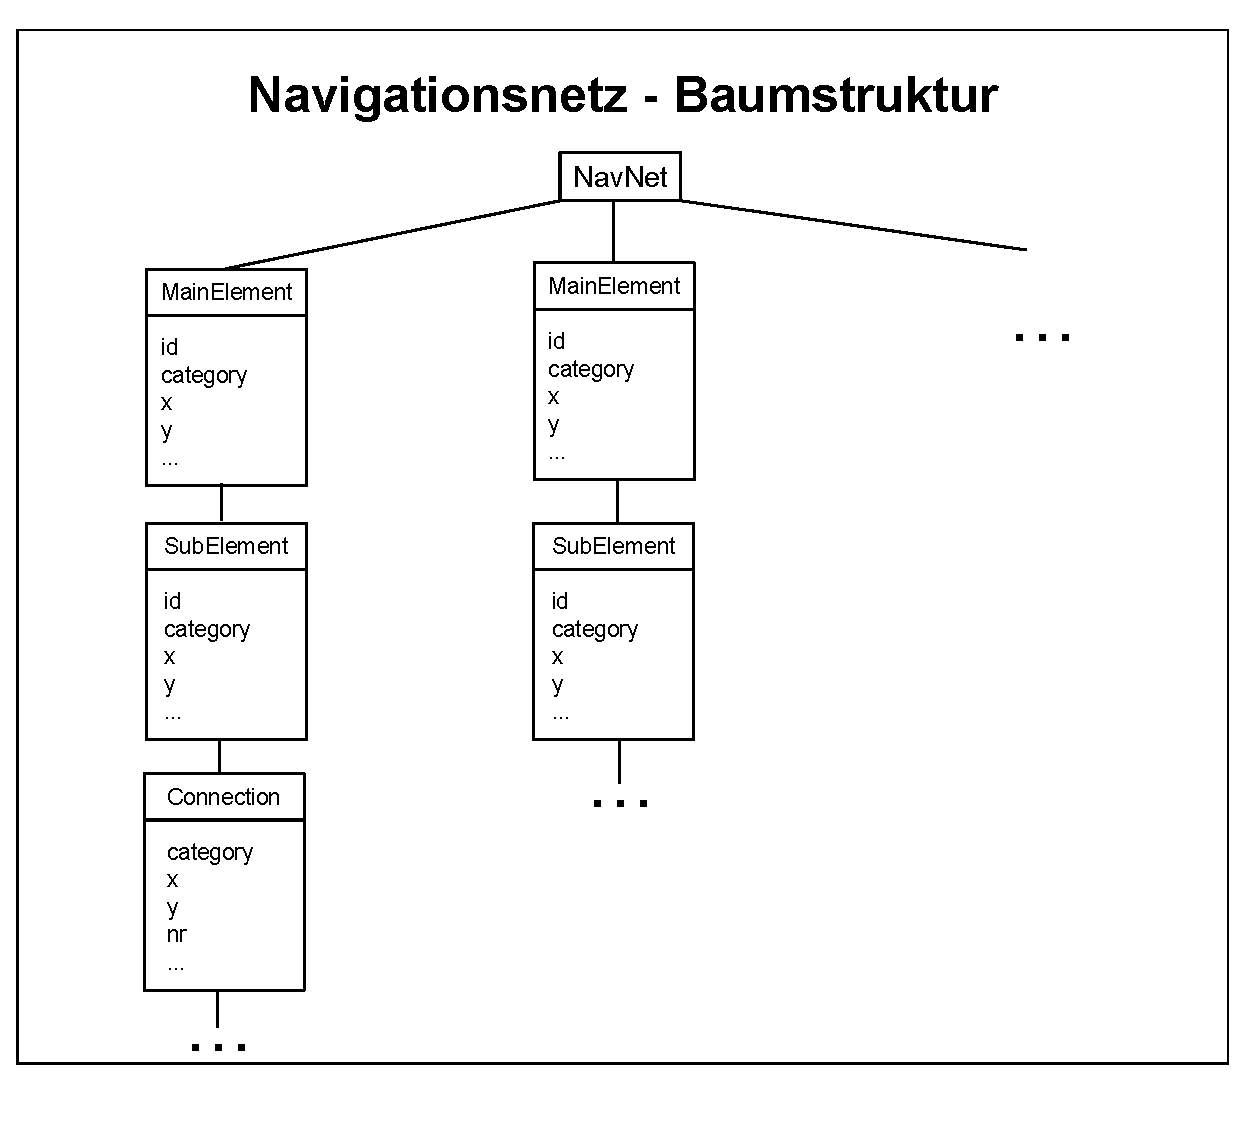
\includegraphics[width=10cm]{figs/baumstruktur}
    \captionbelow{Baumstruktur}
    \label{FIG:baumstruktur}
\end{figure}

\begin{figure}[htbp]
    \centering%
%   \setcapwidth[c]{12cm}%
    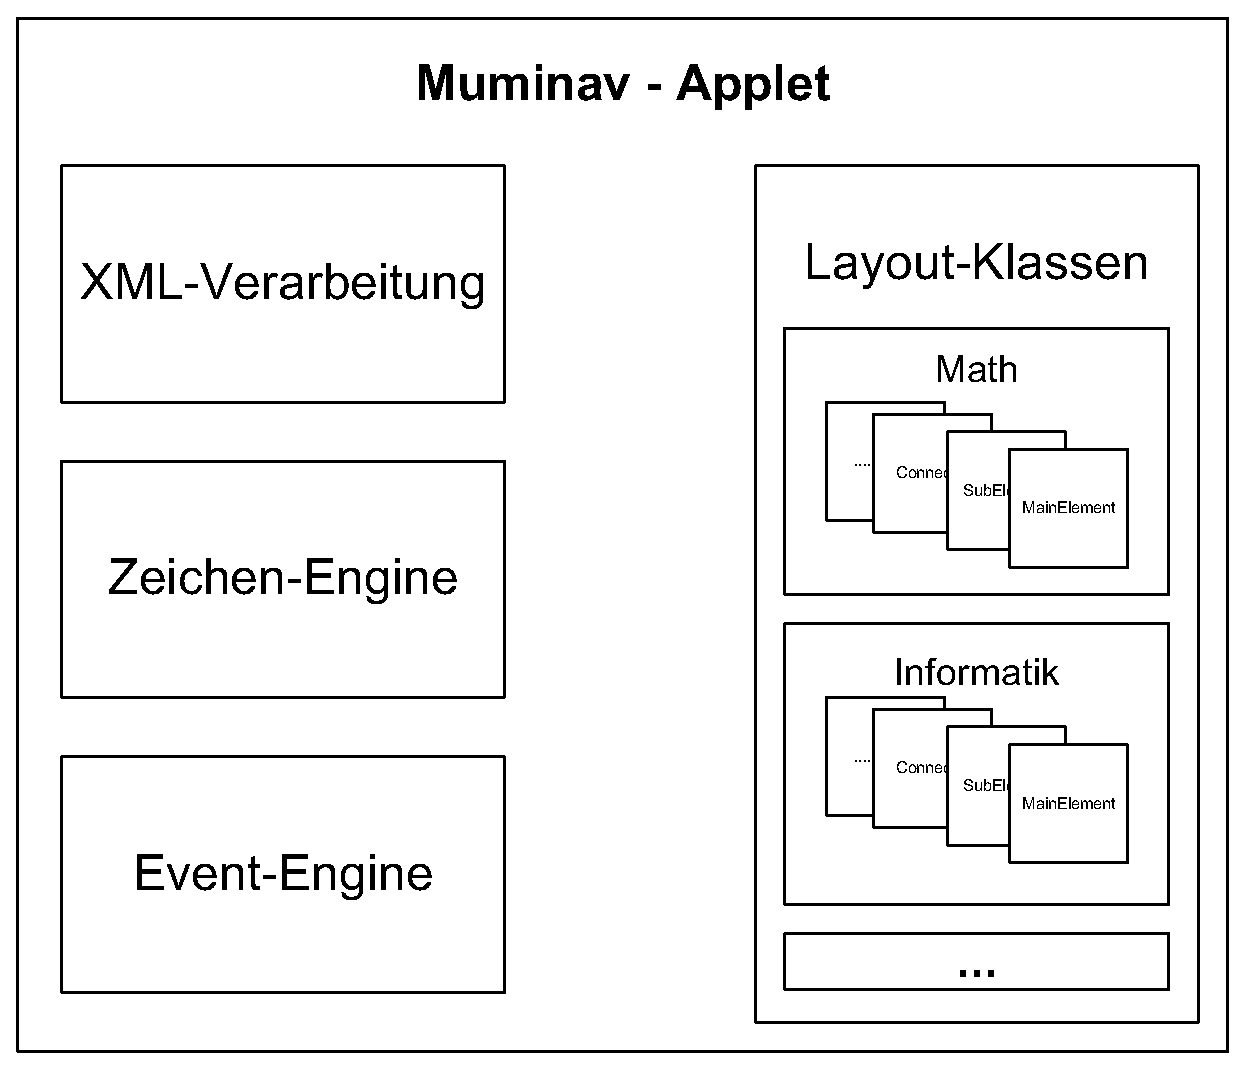
\includegraphics[width=10cm]{figs/aufbau}
    \captionbelow{Aufbau: Haupteile von Muminav}
    \label{FIG:aufbau}
\end{figure}
